\documentclass[12pt,aspectratio=169]{beamer}

\mode<presentation>
{
  \usetheme{Singapore}
  \setbeamersize{text margin left=.6cm,text margin right=.6cm}
%  \setbeamertemplate{navigation symbols}{} % suppress nav bar
%  \setbeamercovered{transparent}
}
\usefonttheme{professionalfonts}
\usepackage{graphicx}
\usepackage{tikz}
\usepackage{amsmath}
\usepackage{mathpazo}
\usepackage[scaled]{helvet}
\usepackage{xcolor,colortbl}
\usepackage{siunitx}

\sisetup{
  number-math-rm=\mathnormal,
  per-mode=symbol
}

\title{Topic 10: Electric Field}
\subtitle{Advanced Placement Physics}
\author[TML]{Dr.\ Timothy Leung}
\institute{Olympiads School}
\date{January 2019}

\newcommand{\pic}[2]{\includegraphics[width=#1\textwidth]{#2}}
\newcommand{\mb}[1]{\mathbf{#1}}
\newcommand{\eq}[2]{\vspace{#1}{\Large\begin{displaymath}#2\end{displaymath}}}


\begin{document}

\begin{frame}
  \maketitle
\end{frame}



\section[Intro]{Introduction}

\begin{frame}{Files for You to Download}
  Download from the school website:
  \begin{enumerate}
  \item\texttt{PhysAP-10-ElectricField.pdf}
  \end{enumerate}
  Please download/print the PDF file before each class. There is no point
  copying notes that are already printed out for you. Instead, take notes on
  things I say that aren't necessarily on the slides. If you want to print
  on paper, I recommend printing 4 pages per side.
\end{frame}



\section[$\mb{F}_q$]{Electrostatic Force}

\begin{frame}{The Charges Are}{Let's Review Some Basics}
  We already know a bit about charge particles:
  \begin{itemize}
  \item A \textbf{proton} carries a \textbf{positive} charge
  \item An \textbf{electron} carries a \textbf{negative} charge
  \item A \emph{net charge} of an object means an excess of protons or electrons
  \item Similar charges are repel, opposite charges attract
  \end{itemize}

  \vspace{.2in}We start with electrostatics:
  \begin{itemize}
  \item Charges that are not moving relative to one another
  \end{itemize}
\end{frame}



\begin{frame}{Coulomb's Law for Electrostatic Force}
  The \textbf{electrostatic force} (or \textbf{coulomb force}) between two
  point charges is given by:

  \eq{-.1in}{
    \boxed{\mb{F}_q=-\frac{kq_1q_2}{r^2}\mb{\hat{r}}_{12}}
  }

  \vspace{-.1in}
  \begin{center}
    \begin{tabular}{l|c|l}
      \rowcolor{pink}
      \textbf{Quantity} & \textbf{Symbol} & \textbf{SI Unit} \\ \hline
      Electrostatic force            & $\mb{F}_q$ &  \si{\newton} (newtons)\\
      Coulomb's constant (electrostatic constant) & $k$   & \si{N.m^2/C^2} \\
      Point charges 1 and 2 (occupies no space) & $q_1$, $q_2$ &
      \si{\coulomb} (coulombs)\\
      Distance between point charges & $r$   & \si{\metre} (meters)\\
      Unit vector of direction between point charges & $\mb{\hat{r}}$ &
    \end{tabular}
  \end{center}

  \vspace{-.1in}
  $\displaystyle k=\frac{1}{4\pi\epsilon_0}=\SI{8.99e9}{N.m^2/C^2}$ where
  $\epsilon_0=\SI{8.85e-12}{C^2/N.m^2}$ is called the
  ``permittivity of free space''
\end{frame}



\section[$\mb{E}$]{Electric Field}

\begin{frame}{Think Electric Field}
  We can get \textbf{electric field} by repeating the same procedure as with
  gravitational field, by grouping the variables in Coulomb's equation:

  \eq{-.2in}{
    F_q=\underbrace{\left[\frac{kq_1}{r^2}\right]}_{E}q_2
  }

  \vspace{-0.1in}
  We can say that charge $q_1$ creates an ``electric field'' ($E$) with an
  intensity

  \eq{-.2in}{
    E=\frac{kq_1}{r^2}
  }

  \vspace{-.1in}The electric field $\mb{E}$ created by $q_1$ is a function
  (``vector field'') that shows how it influences other charged particles
  around it
\end{frame}



\begin{frame}{Electric Field Intensity Near a Point Charge}
  In vector form, the electric field a distance $r$ away from a point charge
  $q_s$ is:

  \eq{-.2in}{
    \boxed{\mb{E}=\frac{kq_s}{r^2}\mb{\hat{r}}}
  }
  \begin{center}
    \begin{tabular}{l|c|c}
      \rowcolor{pink}
      \textbf{Quantity} & \textbf{Symbol} & \textbf{SI Unit} \\ \hline
      Electric field intensity    & $E$   & \si{\newton\per\coulomb} \\
      Coulomb's constant          & $k$   & \si{N.m^2/C^2} \\
      Source charge               & $q_s$ & \si{\coulomb} \\
      Distance from source charge & $r$   & \si{\metre} \\
      Outward unit vector from point source & $\mb{\hat{r}}$ &
    \end{tabular}
  \end{center}
  The direction of the field is radially outward from a positive point charge
  and radially inward toward a negative charge.
\end{frame}



\begin{frame}{Think Electric Field}
  $\mb{E}$ \emph{doesn't do anything} until another charge interacts with it.
  And when there is a charge $q$, the electrostatic force $\mb{F}_q$ that it
  experiences in the presence of $\mb{E}$ is:

  \eq{-.2in}{
    \boxed{\mb{F}_q=\mb{E}q}
  }

  \vspace{-.1in}$\mb{F}_q$ and $\mb{E}$ are vectors, and following the
  principle of superposition, i.e.

  \vspace{-.45in}{\Large
    \begin{align*}
      \mb{F}_q&=\mb{F}_1+\mb{F}_2+\mb{F}_3+\mb{F}_4\ldots\\
      \mb{E}&=\mb{E}_1+\mb{E}_2+\mb{E}_3+\mb{E}_4\ldots
    \end{align*}
  }
  
  \vspace{-.3in}This understanding is especially important when we want to find
  $\mb{F}_q$ and $\mb{E}$ some distance from a continuous distribution of
  charges
\end{frame}



\begin{frame}{Electric Field Lines}
  If you place a positive charge in an electric field, the electrostatic force
  on the charge will be in the direction of the electric field.
  \begin{columns}
    \column{0.25\textwidth}
    \pic{.95}{pos_charge.png}\\
    \pic{.95}{neg_charge.png}
    \column{0.75\textwidth}
    \pic{.95}{2charges.png}
  \end{columns}
\end{frame}



\begin{frame}{Not a Point Charge}
  What if the charge configuration does not consist of point charges?
\end{frame}



\begin{frame}{Lord of the Ring Charge}
  You've been given The One Ring To Rule Them All, and you found out that it is
  charged! What is its electric field at point $P$ along its axis?

  \begin{center}
    \pic{.65}{physicsbook_emism_graphik_35.png}
  \end{center}
\end{frame}



\begin{frame}{Electric Field Along Axis of a Ring Charge}
  \begin{columns}
    \column{.3\textwidth}
    \pic{1.25}{Fig25.jpg}
%    \eq{.05in}{r^2=x^2+a^2}
    \column{.7\textwidth}
    \begin{itemize}
    \item Separate the electric field $d\mb{E}$ from charge $dq$ into
      axial ($dE_x$) and radial ($dE_\perp$) components
    \item Based on symmetry, $dE_\perp$ does not contribute to anything; but
      finding $dE_x$ is straightforward:
    \end{itemize}
  \end{columns}
  \eq{.05in}{
    dE_x =\frac{kdq}{r^2}\cos\theta=\frac{kdq}{r^2}\frac{x}{r}
    =\frac{kxdq}{(x^2+a^2)^{3/2}}
  }      
  Integrating this over all charges $dq$, we have:
  
  \eq{-.2in}{
    E_x =\frac{kx}{(x^2+a^2)^{3/2}}\int dq=\boxed{\frac{kQx}{(x^2+a^2)^{3/2}}}
  }
\end{frame}



\begin{frame}{Electric Field Along Axis of a Uniformly Charged Disk}
  Let's extend what we know to a disk of radius $a$ and charge density $\sigma$
  \begin{columns}
    \column{.3\textwidth}
    \pic{1.2}{serway.png}
    \column{.67\textwidth}
    \begin{itemize}
    \item We start with the solution from the ring problem, and replace $Q$
      with $dq=2\pi\sigma a da$:

      \eq{-.2in}{
        dE_x =\frac{2\pi kx\sigma ada}{(x^2+a^2)^{3/2}}
      }
    \item Integrating over the entire disk:

      \eq{-.3in}{
        E_x =\pi kx\sigma\int\frac{2ada}{(x^2+a^2)^{3/2}}
      }

      \vspace{-.15in}This is not an easy integral!
    \end{itemize}
  \end{columns}
\end{frame}



\begin{frame}{Eclectic Field Along Axis of a Uniformly Charged Disk}
  \begin{columns}
    \column{.3\textwidth}
    \pic{1.2}{serway.png}
    \column{.67\textwidth}
    \begin{itemize}
    \item Luckily for us, the integral is in the form of $\int u^ndu$, with
      $u=x^2+a^2$ and $n=\frac{-3}{2}$.
    \item You can find the integral in any math textbook:

      \eq{-.3in}{
        \boxed{E_x =2\pi k\sigma\left(1-\frac{x}{\sqrt{x^2+R^2}}\right)}
      }
      \end{itemize}
  \end{columns}
\end{frame}



\section{Gauss's Law}

\begin{frame}{Flux}
  \textbf{Flux} is an important concept in many disciplines in physics. The
  flux of a vector quantity $\mb{X}$ is the amount of that quantity flowing
  through a surface. In integral form:

  \eq{-.2in}{
    \Phi=\int\mb{X}\cdot d\mb{A}\quad\text{or}\quad
    \Phi=\int(\mb{X}\cdot\mb{\hat{n}})dA
  }

  The direction of the infinitesimal area $d\mb{A}$ is \textbf{outward normal}
  to the surface.

  \begin{center}
    \pic{.3}{eflux.png}
  \end{center}
\end{frame}



\begin{frame}{Flux}
  \vspace{.2in}$\Phi$ can be something physical, like water, or bananas, or
  something abstract, like electric field (which is what we are interested
  in). We can compute a flux as long as there is a vector field i.e.\
  $\mb{X}=\mb{X}(x,y,z)$.
  In the case of \textbf{electric flux}, the quantity $\mb{X}$ is just the
  electric field, i.e.:
    
  \eq{-.2in}{\Phi_q=\int\mb{E}\cdot d\mb{A}}
  
  \begin{center}
    \pic{.3}{eflux.png}
  \end{center}
\end{frame}



\begin{frame}{Electric Flux and Gauss's Law}
    \textbf{Gauss's law} tells us that if we have a closed surface (think of
    the surface of a balloon), the total electric flux is very well defined:

    \eq{-.2in}{
      \boxed{
        \Phi_\mathrm{total}
        =\oint\mb{E}\cdot d\mb{A}
        =\frac{Q_\mathrm{encl}}{\epsilon_0}
      }
    }
    
    where $Q_\mathrm{encl}$ is the charge enclosed by the surface, and
    $\epsilon_0=\SI{8.85e-12}{C^2/N.m^2}$ is the permittivity of free space.
    That closed surface is called a \textbf{Gaussian surface}.
\end{frame}



\begin{frame}{Electric Field from a Positive Point Charge}
  
  \begin{columns}
    \column{.25\textwidth}
    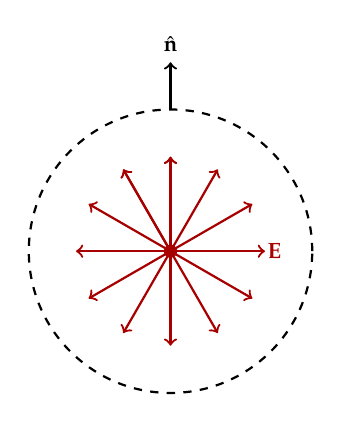
\begin{tikzpicture}[scale=1.2]
      \fill[red!65!black](0,0) circle(0.07);
      \draw[dashed,thick](0,0) circle(1.5);
      \foreach \x in {0,...,13}{
        \draw[red!65!black,thick,rotate=30*\x,->](0,0)--(0,1);
      }
      \draw[thick,->](0,1.5)--(0,2)
      node[pos=1,above]{\footnotesize$\hat{\mb{n}}$};
      \node[red!65!black] at (1.1,0) (E) {\footnotesize$\mb{E}$};
    \end{tikzpicture}
    \column{.75\textwidth}
    By symmetry, electric field lines are radially outward from the charge, so
    the integral reduces to:

    \eq{-.2in}{\Phi=\oint\mb{E}\cdot d\mb{A}=EA=\frac{q}{\epsilon_0}}

    Since area of a sphere is $A=4\pi r^2$, we recover Coulomb's law:

    \eq{-.3in}{ E=\frac{1}{4\pi\epsilon_0}\frac{q}{r^2}=\frac{kq}{r^2}}
    
    In fact, it was through studying point charges that Gauss's law was
    discovered, so it should not be a surprise that they agree.
  \end{columns}
\end{frame}


%\begin{frame}{In Your Homework This Week}
%  In the homework questions this week, you will be asked to find the
%  electric field strength inside and outside of a few common configurations:
%  \begin{itemize}
%  \item Inside \& outside of a spherical shell of charge
%  \item Inside \& outside of a uniformly charged solid sphere
%  \item Near an infinite line charge
%  \item Inside \& outside an infinitely long solid cylinder of charge
%  \item Inside \& outside a cylindrical shell of charge
%  \end{itemize}
%\end{frame}
%
%

\begin{frame}{Electric Field Near an Infinite Plane of Charge}
  \begin{columns}
    \column{.25\textwidth}
    \pic{1.3}{elec_gauss_figure9.jpg}

    \column{.75\textwidth}
    \begin{itemize}
    \item Charge density (charge per unit area) $\sigma$
    \item By symmetry, $\mb{E}$ must be perpendicular to the plane
    \item Our Gaussian surface is a cylinder shown in the left with an area
      $A$; the height of the cylinder is unimportant
    \item We can see that nothing ``flows out'' of the side of the cylinder,
      only at the ends.
    \item The total flux is $\Phi=E(2A)$
    \item The enclosed charge is $Q_\mathrm{encl}=\sigma A$.
    \end{itemize}
  \end{columns}
\end{frame}



\begin{frame}{Electric Field Near an Infinite Plane of Charge}
  \begin{columns}
    \column{.3\textwidth}
    \pic{1.1}{elec_gauss_figure9.jpg}

    \column{.7\textwidth}
    Gauss's law simplifies to:
    
    \eq{-.35in}{
      \oint\mb{E}\cdot d\mb{A}=\frac{Q_\mathrm{encl}}{\epsilon_0}
      \;\;\rightarrow\;\;
      E(2A)=\frac{\sigma A}{\epsilon_0}
    }

    Solving for $E$, we get:

    \eq{-.3in}{\boxed{E=\frac{\sigma}{2\epsilon_0}}}
    \begin{itemize}
    \item $E$ is a constant
    \item Independent of distance from the plane
    \item Both sides of the plane are the same
    \end{itemize}
  \end{columns}
\end{frame}



\begin{frame}{Electric Field between Two Infinite Parallel Plates}
  \begin{center}
    \pic{.6}{elfield-600x205.jpg}
  \end{center}
  \begin{itemize}
  \item\vspace{-.15in}Two plates, each producing an electric field pointing in
    the same direction
  \item The total electric field is twice the value that we found on the last
    slide

    \eq{-.1in}{
      \boxed{E=\frac{\sigma}{\epsilon_0}}
    }
  \end{itemize}
%  \begin{itemize}
%  \item $\mb{E}$ is uniform at all points between the parallel plates,
%    independent of position
%
%  \eq{-.2in}{
%    E\propto\sigma\quad\textsf{\normalsize where}\quad
%    \sigma=\frac{q}{A}
%  }
%  \item $E$ outside the plates is very low (close to zero), except for
%    the fringe effects at the edges of the plates. 
%  \end{itemize}
\end{frame}



%\section[$U_q$ and $V$]{Electric Potential \& Potential Energy}
%
%\begin{frame}
%  \frametitle{Electrical Potential Energy}
%  \framesubtitle{(Follow the Same Work on Gravitational Potential Energy)}
%
%  If we move a charged particle against the electrostatic force, work must be
%  done (either positive or negative, depending on which way the particle moves):
%  
%  \eq{-.3in}{
%    W=\int\mb{F}_q\cdot d\mb{r}
%    =-kq_1q_2\int_{r_1}^{r_2}\frac{dr}{r^2}
%    =-\frac{kq_1q_2}{r}\Big|^{r_2}_{r_1}=-\Delta U_q
%  }
%
%  \vspace{-.1in}\textbf{Electrical potential energy} is defined as:
%    
%  \eq{-.2in}{
%    \boxed{U_q=\frac{kq_1q_2}{r}}
%  }
%
%  \vspace{-.1in}$U_q$ can be (+) or (-), because charged particles can be
%  either (+) or (-)
%\end{frame}
%
%
%
%
%\begin{frame}
%  \frametitle{How it Differs from Gravitational Potential Energy}
%  \begin{columns}
%    \column{.33\textwidth}
%    \begin{center}
%      Two positive charges:
%
%      \eq{-.3in}{U_q>0}
%    \end{center}
%    
%    \column{.33\textwidth}
%    \begin{center}
%      Two negative charges:
%
%      \eq{-.3in}{U_q>0}
%    \end{center}
%    
%    \column{.34\textwidth}
%    \begin{center}
%      One positive and one negative charge:
%
%      \eq{-.5in}{U_q<0}
%    \end{center}
%  \end{columns}
%
%  \vspace{.2in}
%  \begin{itemize}
%  \item $U_q>0$ means positive work is done to bring two charges together from
%   $r=\infty$ to $r$ (both charges of the same sign)
%  \item $U_q<0$ means negative work (the charges are opposite signs)
%  \item For gravitational potential $U_g$ is always $<0$
%  \end{itemize}
%\end{frame}
%
%\begin{frame}
%  \frametitle{Electric Potential}
%  \framesubtitle{Start with an Analogy}
%
%  When I move an object of mass $m$ against a gravitational force from one
%  point to another, the work that I do is directly proportional to $m$, i.e.\
%  there is a ``constant'' in that scales with \emph{any} mass, as long as they
%  move between those same two points:
%
%  \eq{-.25in}{W=\Delta U_g=Km}
%
%  \vspace{-.15in}In the trivial case (small changes in height, no change in
%  $g$), this constant is just
%
%  \eq{-.15in}{
%    \frac{\Delta U_g}{m}=g\Delta h
%  }
%
%  \vspace{-.1in}(We have actually looked at this briefly in our discussion on
%  universal gravitation.)
%\end{frame}
%
%
%\begin{frame}
%  \frametitle{Electric Potential}
%
%  This is also true for moving a charged particle $q$ against an electric
%  electric field created by $q_s$, and the ``constant'' is called the
%  \textbf{electric potential}. For a point charge, it is defined as:
%
%  \eq{-.3in}{
%    \boxed{V=\frac{U_q}{q}=\frac{kq_s}{r}}
%  }
%
%  The unit for electric potential is a \emph{volt} which is
%  \emph{one joule per coulomb}:
%
%  \eq{-.25in}{
%    \SI{1}{\volt}=\SI{1}{\joule\per\coulomb}
%  }
%
%  \vspace{-.15in}We can easily that there is also a relationship between
%  electrical potential $V$ and electric field $\mb{E}$:
%  
%  \eq{-.3in}{
%    \boxed{\Delta V=\int\mb{E}\cdot d\mb{r}}
%  }
%\end{frame}
%
%
%
%\begin{frame}
%  \frametitle{Potential Difference (Voltage)}
%
%  The change in electric potential is called the
%  \textbf{electric potential difference} or \textbf{voltage}:
%
%  \eq{-.2in}{
%    \boxed{\Delta V=\frac{\Delta U_q}{q}}\quad\textsf{\normalsize and}\quad
%    \boxed{dV=\frac{dU_q}{q}}
%  }
%
%  Here, we can relate $\Delta V$ to an equation that we knew from Physics 11,
%  which related to the energy dissipated in a resistor in a circuit
%  $\Delta U$ to the voltage drop $\Delta V$:
%    
%  \eq{-.2in}{
%    \boxed{\Delta U_q=q\Delta V}
%  }
%
%  Electric potential difference also has the unit \emph{volts} (\si{\volt})
%\end{frame}
%
%
%
%\begin{frame}
%  \frametitle{Getting Those Names Right}
%  Remember that these three quantities are all scalars, as opposed to
%  electrostatic force $\mb{F}_q$ and electric field $\mb{E}$ which are vectors
%
%  \vspace{.1in}
%  \begin{itemize}
%  \item Electric potential energy:
%    \begin{displaymath}
%      U=\frac{kq_1q_2}{r}
%    \end{displaymath}
%  \item Electric potential:
%    \begin{displaymath}
%      V=\frac{kq}{r}
%    \end{displaymath}
%  \item Electric potential difference (voltage):
%    \begin{displaymath}
%      \Delta V=\frac{\Delta U_q}{q}
%    \end{displaymath}
%  \end{itemize}
%\end{frame}
%
%
%\begin{frame}
%  \frametitle{Relating $U_q$, $\mb{F}_q$ and $\mb{E}$}
%  \framesubtitle{Our Integrals In Reverse}
%  Using vector calculus, we can relate electrostatic force ($\mb{F}_q$) to
%  electric potential energy ($U_q$), and electric field ($\mb{E}$) to the
%  electric potential ($V$):
%
%  \eq{-.2in}{
%    \mb{F}_q=-\nabla U_q=-\frac{\partial U_q}{\partial r}\hat{\mb{r}}
%    \quad\;\;
%    \mb{E}=-\nabla V=-\frac{\partial V}{\partial r}\hat{\mb{r}}
%  }
%
%  \begin{itemize}  
%  \item\vspace{-.2in}Electrostatic force $\mb{F}_q$ always points from high
%    potential to low potential energy
%  \item Electric field can also be expressed as the change of electric
%    potential per unit distance, which has the unit
%    
%    \eq{-.25in}{
%      \SI{1}{\newton\per\coulomb}=\SI{1}{\volt\per\metre}
%    }
%  \item Electric field is also called ``potential gradient''
%  \end{itemize}
%\end{frame}
%
%
%
%\begin{frame}
%  \frametitle{Equipotential Lines}
%  \begin{center}
%    \pic{0.65}{plate3.png}
%  \end{center}
%
%  \vspace{-.2in}The dotted blue lines are called \textbf{equipotential lines}.
%  They are always \emph{perpendicular} to the electric field lines. Charges
%  moving in the direction of the equipotential lines have constant electric  potential
%\end{frame}
%
%\begin{frame}
%  \frametitle{Electric Field and Electric Potential Difference}
%  
%  The relationship between electric field ($\mb{E}$) and electric potential
%  difference ($V$):
%    
%  \eq{-.15in}{
%    \mb{E}=-\frac{\partial V}{\partial r}
%  }
%
%  In a uniform electric field (e.g.\ parallel plate) it simplifies to a very
%  simple equation:
%
%  \eq{-.2in}{
%    \boxed{E=\frac{\Delta V}{d}}
%  }
%
%  \vspace{-.1in}
%  \begin{center}
%    \begin{tabular}{l|c|l}
%      \rowcolor{pink}
%      \textbf{Quantity} & \textbf{Symbol} & \textbf{SI Unit} \\ \hline
%      Electric field intensity & $E$ & \si{\newton\per\coulomb}
%      (newtons per coulomb) \\
%      Electric potential difference between plates & $\Delta V$ &
%      \si{\volt} (volts) \\
%      Distance between plates       & $d$ & \si{\metre} (meters)\\
%    \end{tabular}
%  \end{center}
%\end{frame}
%
\end{document}
